\ifdefined\included
\else
\setcounter{chapter}{2} %% Numéro du chapitre précédent ;)
\dominitoc
\faketableofcontents
\fi

\chapter{Ontologenius: A long-term semantic memory}
\chaptermark{Ontologenius}
\label{chap:ontologenius}
\minitoc

In this chapter, we present the software Ontologenius. It is a lightweight and open-source software to store ontology, perform reasoning on, update it, and query it. At the difference of other software, Ontologenius has been developed especially for \acrlong{hri} application. In this way, it is able to manage several ontology instances in parallel and put a focus on the concepts' names in natural language. It aims to be used as a server, common to an entire robotic architecture, providing consistent and always up to date knowledge to any other component of the architecture. Consequently, it is thread-safe and can be queried by several components at a time while being constantly updated.

An earlier stage of this contribution had been presented and publish at the RO-MAN 2019 conference~\cite{sarthou_2019_ontologenius}. Due to the evolution of the software since this publication, the current chapter presents new features and a more mature contribution.

\section{Design and features}

In this section, we first explain our choice to use ontology as a means of representing knowledge, both from the point of view of its expressiveness and its growing use in robotics. Then, we present the wanted features for software managing such an ontology and the level of expressiveness we have selected for this software. Finally, we draw a formalism of the kind of ontology we use all along this thesis.

\subsection{Why an ontology?}

In cognitive psychology, we saw that semantic memory refers to the encyclopedic knowledge of words associated with their meanings. After several studies, by studying, among other things, participant response times to questions, some authors have proposed a model of this semantic memory as being a semantic network~\cite{collins_1969_retrieval, collins_1970_does}. With this model, they put the hypothesis that knowledge is organized in a hierarchic way, respecting a principle of inclusion among classes. For example, a class representing the concept of cat would inherit an upper class, representing the concept of animal. In addition, instances of these classes would be linked to others through properties, and in the same way, as for the classes, a notion of hierarchy over the properties would exist. Such a structure of knowledge in humans would allow a cognitive economy as well as efficient storage of this knowledge. Even if not the first to formalize the principle of a semantic network, Collins and Quillian have provided prominent works and computer implementations.


As reported in~\cite{prasad_2020_knowledge}, such a semantic network, also call semantic graph or knowledge graph, is today frequently used as knowledge representation in robotic application to represent among others:

\begin{itemize}
  \item the categories of entities at diffrent level of abstraction~\cite{balint_2018_variations}, like a handle is a physical object
  \item the carateristics of entities~\cite{tenorth_2017_representations}, like a fidge has a handle
  \item the function or purpose of entities~\cite{paulius_2019_functional}, like the fridge handle allows to open the fridge
  \item the location of an entity regarding an other one (i.e. spatial relations)~\cite{singh_2020_fuzzy}, like the bottle milk is in the fridge
\end{itemize}

%This initial model has since been formalized as an ontology \cite{berners-lee_semantic_2001} and is already widely used in the semantic web.

\subsection{Desired features}

\subsection{Ontology formalism}
\label{sec:kb_formalism}

Even if we saw that the use of ontology is today a common way to represent semantic knowledge, we will recall in this subsection the composition of an ontology. For each element composing it, we will draw a formalization based on Description Logic (DL), then give examples using the Turtle syntax. The pieces of ontologies used in the examples of this subsection are voluntarily simplified. The introduced notations will be the ones used in the rest of this thesis and the graphical representations, both in terms of color and form, will be used as often as possible.

On the base of the definition of a Description Logic ontology presented in \cite{fokoue_2006_summary} and \cite{krotzsch_2013_description}, we define a semantic knowledge base $\kbs$ represented as an ontology by  $\kbs = \langle \Abox, \Tbox, \Rbox \rangle$. $\Abox$, $\Tbox$, and $\Rbox$ are respectively called the ABox, TBox, and RBox of the ontology. In the Description Logic knowledge base it is common to only find the ABox, containing extensional knowledge (general knowledge about a domain), and the TBox containing intensional knowledge (instantiated knowledge)~\cite{baader_2003_description}. The first describes the terminology while the latter contains assertions. The definition we choose to base on extracts a part of the TBox to put it into the RBox making it clearer.

\subsubsection{The ontology TBox: Terminological Knowledge}

\begin{figure}[ht!]
\centering
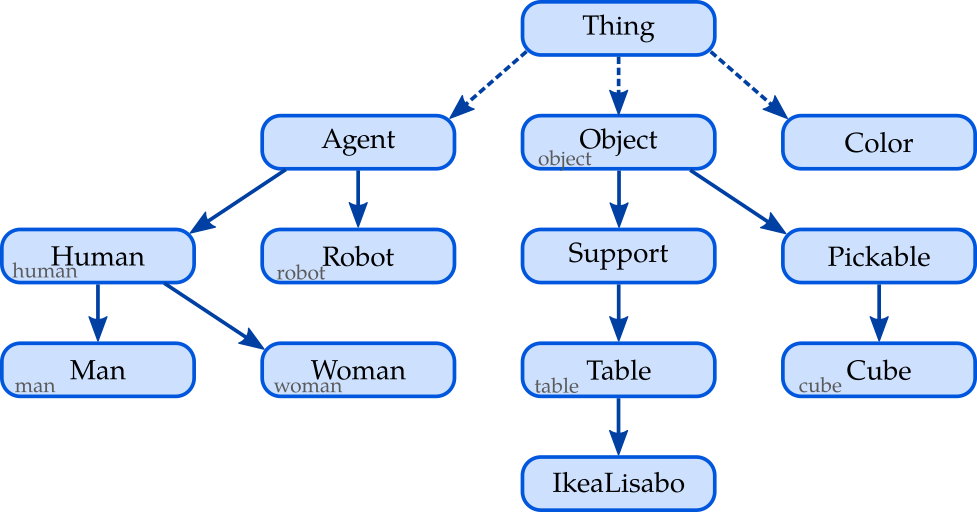
\includegraphics[scale=0.4]{figures/chapter2/Tbox.png}
\caption{\label{fig:Tbox} Representation of an ontology class hierarchy graph to illustrate the composition of a TBox. Taking the class Human, the bottom arrow has to be read as \textit{``A man is a kind of Human''}. The texts at the bottom left of the class, if there is, are the classes' labels in natural language.}
\end{figure}

\improvement{Itemize}
The TBox $\Tbox$ contains assertions about the \textbf{classes} (types) of the ontology. It is defined by $\Tbox = \langle \classset, H \rangle$. It can be seen as a directed acyclic graph as presented in Figure~\ref{fig:Tbox}. $\classset$ is the set of all the classes of the ontology. In our example, $\classset = \{Thing,\ Agent,\ Object, ...,\ IkeaLisabo\}$. Considering the TBox as a graph, $H$ stores its directed edges. They represent the inheritance links between the classes (i.e. the subsumption assertions). We often use the special property ``isA'' to refer to these links (e.g. \textit{(Human, isA, Agent)}). In the OWL language, they are described with the property rdfs:subClassOf, as illustrated in the Listing~\ref{lst:Tbox}.

\noindent
\begin{minipage}{\textwidth}
\begin{lstlisting}[frame=single, basicstyle=\scriptsize\ttfamily, label={lst:Tbox}, caption={Description of ontology classes in the OWL language using the Turle syntax.},captionpos=b, style=OwlTurtle]
:Human rdf:type owl:Class ;
       rdfs:subClassOf :Agent .

:Man   rdf:type owl:Class ;
       rdfs:subClassOf :Human .
\end{lstlisting}
\end{minipage}

\subsubsection{The ontology RBox: Relations between Roles}

\begin{figure}[ht!]
\centering
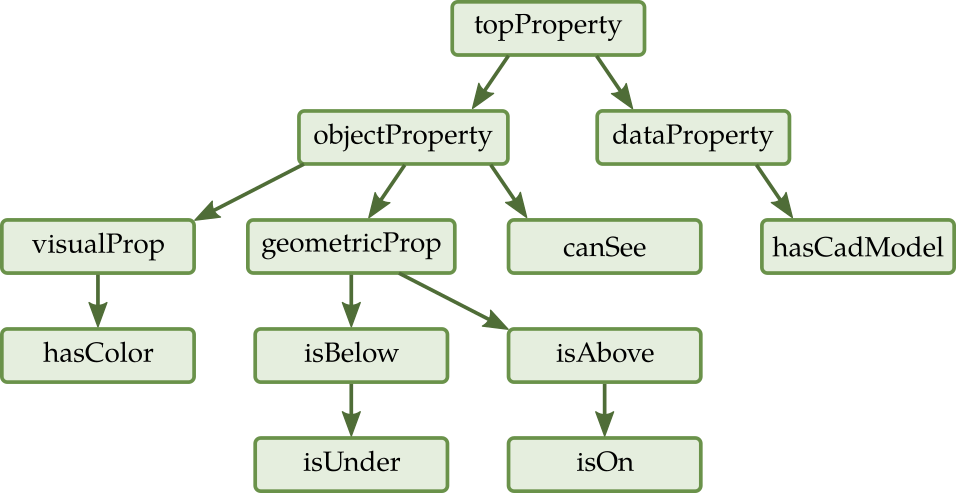
\includegraphics[scale=0.4]{figures/chapter2/Rbox.png}
\caption{\label{fig:Rbox} Representation of an ontology property hierarchy graph to illustrate the composition of an RBox. Taking the property isBelow, the bottom arrow has to be read as: \textit{``The property isUnder is a specification of the property isBelow''}.}
\end{figure}

The RBox $\Rbox$ contains axioms about the \textbf{properties} (roles). It is at least defined by $\Rbox = \langle \propset, \inclset, \invset, \domainset, \rangeset \rangle$. In the same way as the TBox, $\propset$ is the set of properties, and $\inclset$ stores the directed edges of the finite directed acyclic graph representing the inheritance links between the properties. Such a graph is represented in Figure~\ref{fig:Rbox}. These inheritance links aim at specifying properties. In our example, the property IsOn is a specification of the property isAbove in the way that an object being on another is an object that is above the latter and being in contact with. It is described with the property rdfs:subPropertyOf in the OWL language. 
$\invset = \{(\property, \property^{-1}) \in \propset^2\}$ is the set representing the properties inverses (\textit{e.g.} $(isOn, isUnder) \in Inv$). Describing the inverse of a property is useful first to reduce description work since if some describe a relation involving a property for which an inverse is defined, the inverse relation is also described in an underlying way. Moreover, for an algorithm exploring an ontology, knowing that a relation uses a property having an inverse can allow reducing the algorithm complexity by not considering the inverse relation into the exploration.
Finally, $\domainset$ and $\rangeset$ are two sets representing respectively the properties domains and ranges. Their are define by $\domainset = \{(\property, \class)\}$ and $\rangeset = \{(\property, \class)\}$ with $\property \in \propset$ a property and $\class \in \classset$ a class. The domain of a property informs on the type of resources that may use the property, thus the type of the subject of a triplet. The range of a property informs on the valid values applied to the property, thus the type of the object of a triplet. For the property isOn, we would therefore have $(isOn,\ Object) \in \domainset$ and $(isOn,\ Support) \in \rangeset$. In this way, we state that the property IsOn can be used to describe that an object is on top of an object being support. Domains and ranges can be used in two ways. It can be to check the consistency of an ontology by checking if the way the properties have been used corresponds to their definition. It can also be used to reason on the ontology and extract new knowledge from a given situation. If, for example, an entity is said to be on top of another that is not described as being a support, we could deduce that this second entity may be a support.

The formalization above considers only a general kind of property while the OWL language makes the distinction between two main categories. The \textbf{object properties}, linking two entities, and \textbf{data properties}, linking an entity to a value. While both are slightly different, we will only keep a general definition of a property for our formalization to simplify the future algorithm explanations. An example of the description of an object property and a data property from the Figure~\ref{fig:Rbox} are illustrated in the Listing~\ref{lst:Rbox} using the OWL language.

\begin{lstlisting}[frame=single, basicstyle=\scriptsize\ttfamily, label={lst:Rbox}, caption={Description of ontology properties in the OWL language using the Turle syntax.},captionpos=b, style=OwlTurtle]
:isOn  rdf:type owl:ObjectProperty ;
       rdfs:subPropertyOf :isAbove ;
       owl:inverseOf :isUnder ;
       rdfs:domain :Object ;
       rdfs:range :Support .

:hasCadModel rdf:type owl:DatatypeProperty ;
             rdfs:domain :Object .
\end{lstlisting}

\subsubsection{The ontology ABox: Asserting facts}

\begin{figure}[ht!]
\centering
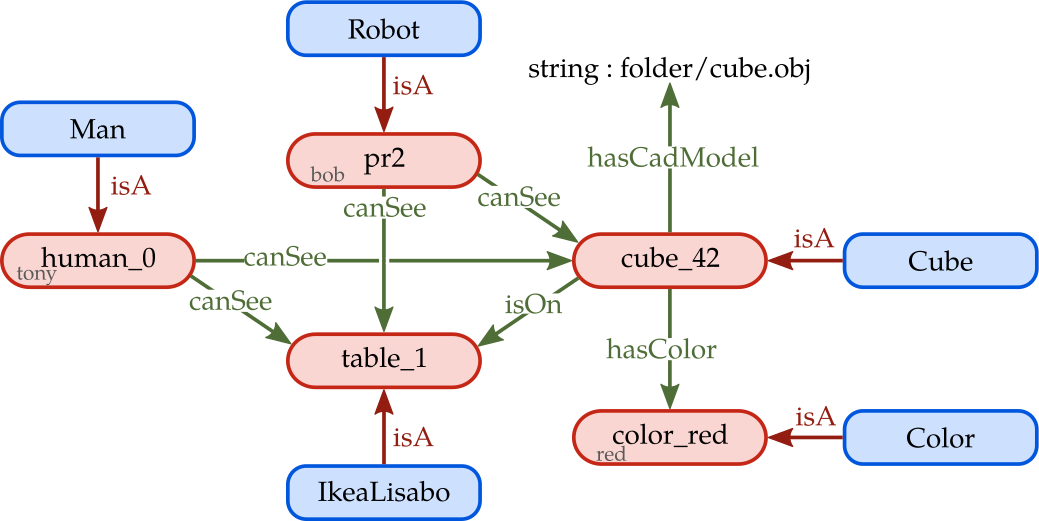
\includegraphics[scale=0.4]{figures/chapter2/Abox.png}
\caption{\label{fig:Abox}  Representation of an ontology instances graph to illustrate the composition of an ABox. Red boxes are individuals of the ontology. Green arrows are properties coming from the RBox and applied to individuals. Red arrows represent a direct inheritance link between an individual and a class coming from the TBox. The texts at the bottom left of the individuals, if there is, are the individuals' labels in natural language.}
\end{figure}

The ABox $\Abox$ contains assertions about the \textbf{entities} (individuals) of the ontology. When we refer about entities, we no more speak about general concepts but rather of instantiated concept, being either a physic or virtual entity. The ABox is defined by $\Abox = \langle \indivset, \inheritset_0, \relationset \rangle$. $\indivset$ is the set of all the entities represented in the ontology. $\inheritset_0$ the set of direct types of $\indivset$ such as $\inheritset_0 = \{(\indiv, \class) \}$ with $\indiv \in \indivset$ an individual and $\class \in \classset$ a class. In the graphical representation of an ABox in the Figure.~\ref{fig:Abox}, the red blocks are the ABox entities ($\indivset = \{human_0,\ pr2,\ ...,\ table\_1\}$) and the red arrows with the label ``isA'' are the intities direct types ($(cube\_42, Cube) \in \inheritset_0$).
$\relationset$ is finally the set of \textbf{relations} between entities. Such relation are in the form of triplets $(\subject, \property ,\object)$ where $\subject$ is the subject, $\property$ the property and $\object$ the object. The set of relations is thus defined by $\relationset = \{(\subject, \property ,\object) | (\subject, \object) \in \indivset^2, \property \in \propset\}$. These relations are represented by the green arrows between the entities in Figure~\ref{fig:Abox}. We can note in this figure the presence of the use of a data property ``hasCadModel''. This property does not link two entities, which goes against the previous definition. Regarding our formalization and to keep it tractable, we can however keep it as it is, and view the string value as an entity having for direct type a concept ``String''. An example of the description of an entity from the Figure~\ref{fig:Abox} is illustrated in the Listing~\ref{lst:Abox} using the OWL language.

\begin{lstlisting}[frame=single, basicstyle=\scriptsize\ttfamily, label={lst:Abox}, caption={Description of an ontology individual in the OWL language using the Turle syntax.},captionpos=b, style=OwlTurtle_indiv]
:cube_42  rdf:type     :Cube ;
          :hasColor    :color_red ;
          :hasCadModel ``folder/cube.obj''^^string ;
          :isOn        :table_1 .
\end{lstlisting}

We just saw that in the ABox, $\inheritset_0$ contains the direct types of entities. We also saw that the classes can inherit from one each other in the TBox, thanks to the classes inheritance directed edges stored in $H$. This means that the individuals of the ABox have inherited types. Taking the entity cube\_42 of Figure.~\ref{fig:Abox}, its direct type is the class Cube ($(cube\_42,\ Cube) \in \inheritset_0$). Regarding the TBox represented in Figure.~\ref{fig:Tbox}, a Cube is a kind of Pickable ($(Cube,\ Pickable) \in H$), itself being a kind of Object ($(Pickable,\ Object) \in H$). We can thus say that the entity cube\_42 is a Cube, a Pickable, and an Object. To represent it, we use $\inheritset$ to denote the set of direct and inherited types. We thus have $\{ (cube\_42,\ Cube), (cube\_42,\ Pickable), (cube\_42,\ Object)\} \subset \inheritset$.

\subsubsection{Extending the ontology TBox}

With the use of the relation set $\relationset$ of the ABox we saw that we can apply properties to individuals to link them together and form relations in the form of triplets. However, some could want to apply properties to classes to describe general links between classes. While properties domains and ranges already give such relations this can be not enough. Taking an object property hasMother, we can assign to it the class Human for domain and Woman for range. With such description, we state that a human CAN have a mother that is a woman but we do not describe that even if we do not know how it is, a human has a mother how is a woman. For this particular example, we could use cardinality constraint but we will not go as far. Taking now the data property hasCadModel of Figure~\ref{fig:Rbox}, we have applied it to a specific entity in the example of Figure~\ref{fig:Abox}. But what about a Table Lisabo (IkeaLisabo in Figure~\ref{fig:Tbox})? Any table of this model will have the same CAD model and we do not want to put this relation to every entity of this type of table. Here domains and range are not sufficient to represent it. To do so, we will use \textbf{annotation properties} applied to classes. Annotation properties are usually used to document ontologies and not to describe general relations on classes. We take thus some liberty regarding the OWL standard for convenience. However, we will try to use it in very particular cases where no other simple solution can be applied. Relations to classes using annotation properties are thus added to the definition of a TBox $\Tbox = \langle \classset, H, \annotationset \rangle$, where $\annotationset$ is the set of relation between classes in the form of triplets.

\subsubsection{Advanced use of properties}

In this sub-section, we present a formalism of an ontology in the form of $\kbs = \langle \Abox, \Tbox, \Rbox \rangle$. All the knowledge stored in $\kbs$ are sufficient to build exploration algorithm on top of it. However, to reason on ontology aditional descriptions are necessary in the form of properties characteristics. We do not add them to the knowledge base formalism but enumerate them bellow: 

\begin{itemize}
	\item \textbf{Symmetric property}: If the relation $(x, p, y)$ holds in $\relationset$ with $p$ being a symmetric property, the relation $(y, p, p)$ is also part of $\relationset$. \\ $hasSpouse$
	
	\item \textbf{Asymmetric property}: If the relation $(x, p, y)$ holds in $\relationset$ with $p$ being an asymmetric property, the relation $(y, p, p)$ can no be part of $\relationset$. \\ $hasChild$
	
	\item \textbf{Reflexive property}: A reflexive property can be used to link an individual to itself. \\ $hasRelative$
	
	\item \textbf{Irreflexive property}: An irreflexive property can not be used to link an individual to itself. \\ $hasParent$
	
	\item \textbf{Functional property}: Every individual can be linked by a functional property to at most one other individual. By this way, if ${(x, p, y), (x, p, z)} \subset \relationset$, then $y = z$. \\ $hasFather$
	
	\item \textbf{Inverse functional property}: Every individual can holds an iverse functional property at most one. By this way, if ${(x, p, y), (z, p, y)} \subset \relationset$, then $x = z$. \\ $hasHusband$
	
	\item \textbf{Transitive property}: A transitive property describe a link between two individuals x and z whenever it exist a link between x and y, and y with z with this property. If ${(x, p, y), (y, p, z)} \subset \relationset$ with p a transitive property, then $(x, p, z) \in \relationset$. \\ $hasAncestor$
	
	\item \textbf{Property chain axiom}: While the transitive property characteristic decsribe a link between several individuls with the same property, the chain axiom does the same with distinct properties. Given the chain $p_1 \bullet p_2 \Rightarrow p_3$, if ${(x, p_1, y), (y, p_2, z)} \subset \relationset$, then $(x, p_3, z) \in \relationset$. \\ $hasParent \bullet hasParent \Rightarrow hasGrandparent$
	
	\item \textbf{Disjunction}: Given two disjoint elements (classes or properties), a third element can not inherit of the both disjoint elements. \\ $Man \sqcup Woman$
\end{itemize}

\subsubsection{Labeling functions}

We saw in the previous chapter that the semantic knowledge base is part of what we assimilate to be the declarative memory. The particularity of such memory is the ability to speak about the knowledge it stores. In this way, we introduce a labeling function $\labelfunc$ for any element of the ontology. This labeling function is specified for the individuals ($\alabel$), the classes ($\tlabel$), and the properties ($\plabel$). Considering the individuals labeling function $\alabel: \indivset \rightarrow Lbl$ with $Lbl$ a set of communicable names encoded as UTF8 string in our implementation. The same holds for the other two labeling functions.

\subsubsection{Ontology for Human-Robot Interaction}

Because we are working in the field of Human-Robot Interaction, it is mandatory for the robotic agent to be able to represent its own knowledge but also to represent an estimate of its human partners' knowledge. Such features will be explained later in this thesis and we only introduce the related notation for the moment.
We define the robot's own simbolic knowledge base $\kbs^R = \langle \Abox^R, \Tbox^R, \Rbox^R\rangle$.
Then, for each human agent $H_i$ the robot knows, we concider the agent's semantic knowledge $\kbs^{H_i} = \langle \Abox^{H_i}, \Tbox^{H_i}, \Rbox^{H_i} \rangle$.
The robot's global knowledge thus encompasses both its own semantic representation of the environment as well as an \textbf{estimation} of the other agent's knowledge.
In the rest of this thesis, we will simply use the notation $\kbs$ in cases where the used knowledge base does not matter.

\subsubsection{Ontology formalism recap}

The ontology definition used all along this thesis is summarized in Table~\ref{tab:onto_symboles}.

\begin{table}[ht!]
\caption{The list of symbols of used to define a semantic knowledge base as an ontology }
\label{tab:onto_symboles}
\begin{tabular}{ll}
{\ul \textbf{$\Abox$ ABox entities/indiv}} & {\ul \textbf{$\Tbox$ TBox classes/concepts}}  \\
$\indivset$: set of entities               & $\classset$: set of classes  \\
$\inheritset_0$: entities' direct types        & $H$: classes inheritance links \\
$\relationset$: relations between entities    & $\annotationset$: relations between classes  \\
$\alabel$: individuals labeling function & $\tlabel$: classes labeling function \\
 & \\
\multicolumn{2}{l}{{\ul \textbf{$\Rbox$ RBox roles/properties}}}                          \\
$\propset$: set of properties              &                                              \\
$\inclset$: properties inheritance links       & $\invset$: properties inverses                   \\
$\domainset$: properties' domains sets     & $\rangeset$: properties' ranges sets   \\
$\plabel$: properties labeling function & \\
\end{tabular}
\end{table}

\section{Architecture}

\subsection{Permanent versus temporary data structure}

\subsection{Concepts' identifier versus name in natural language}

\subsection{Resoning to enrich the knowledge}



\section{Managing others' estimated knowledge}

\subsection{Ontologenius multi-instances principle}

\subsection{Catching knowledge at a given moment}

\subsection{Exploring several possible mental states at once}



\section{Using Ontologenius in robotic applications}

\subsection{Inserting new knowledge}

\subsection{Retrieving knowledge}

\subsubsection{Low-level queries}

\subsubsection{SPARQL-like interface}

\subsection{The Application Programming Interface}

\subsubsection{Debbuging tool}



\section{Computational preformance evaluation}

In this section, we evaluate the Ontologenius performance and scalability through comparison with two systems and using their own tests. First, we compare with the KnowRob system with a focus on required CPU time to insert new knowledge and required memory to store this knowledge. The second system of comparison is ORO. With this latter, we measure query resolution time. Finally, we present some additional measures like concept recovery time and \sparql{} query resolution time.

\subsection{Comparing with Knowrob}

We start these comparisons with the KnowRob system presented in~\cite{tenorth_2013_knowrob}. This system is composed of several modules able to perform dedicated reasoning like temporal reasoning, CAD model segmentation, or object perception. All these modules are integrated around the logical programming language SWI Prolog~\cite{wielemaker_2012_swi}. OWL ontologies are loaded using the SWI Prolog’s Semantic Web library~\cite{wielemaker_2003_prolog} which provide a performant and scalable way to manipulate RDF structure in Prolog. Internally, the triple structure of the ontologies is represented as Prolog predicates. At the difference of Ontologenius, the Prolog system and thus KnowRob does not aim to be used as a server but rather as a monolithic and highly integrated system. To provide a fair comparison, in the part, we used Ontologenius without the ROS communication layer. Consequently, a single process runs both ontologenius and the test application.

The article~\cite{tenorth_2017_representations} propose a detailed presentation of the internal representation of KnowRob and present some performance and scalability analysis. The following comparisons have to be considered carefully. KnowRob is a wider and more mature system than Ontologenius. It proposes more advanced capability in terms of reasoning and integration. Ontologenius is more focused on \acrshort{hri} applications as presented earlier in this section. In this way, some simplifications that have been done to fit at our best the KnowRob tests may impact the results. The final reason why the following results should be taken with caution is that due to the complexity of the KnoRob system, we did not perform their test on our end. The results for the KnowRob system comes from their paper~\cite{tenorth_2017_representations}. Consequently, in this section, we do not aim at showing that Ontologenius is "better" than KnowRob. We rather want to show that Ontologenius is not out of the scope in terms of performance and scalability regarding a well-established software.

For the tests we have replicated, they use the description of visual perception entities. Such an entity represents the occurrence of the perception of a given object, having a given pose at a given instant. An example of one of these entities is illustrated in listing~\ref{lst:chap2_visual_perception}. The entity $cup\_i$ is the perceived object. The entity $VisualPerception\_i$ is the perception occurrence. It uses an object property to make a link with the perceived object and two data properties to represent the object's pose and the perception time stamp. The first simplification we had to make is the representation of the matrix of position. In Ontologenius, the data types are only represented in a serialized way as no internal manipulation of these types are made. Thanks to the use of Prolog, KnowRob can manipulate such a matrix and perform operations on it. Even if it is not said if they have inverse properties or not, we add one for the \textit{objectActedOn} property in order to know in which perception instance an object has been perceived.

\begin{lstlisting}[frame=single, basicstyle=\scriptsize\ttfamily, label={lst:chap2_visual_perception}, caption={Description of a visual perception entity created in a somparable way as in the Knowrob system. The description is provided in the OWL language using the Turle syntax.},captionpos=b, style=OwlTurtle_indiv]
:cup_i  rdf:type   :Cup ;

:VisualPerception_i  rdf:type         :VisualPerception ;
                     :objectActedOn   :cup_i ;
                     :eventOccursAt   [[1,0,0,2.56], ... ,[0,0,0,1]]^^RotMat ;
                     :startTime       6572^^Time .
\end{lstlisting}

\begin{figure}[ht!]
\centering
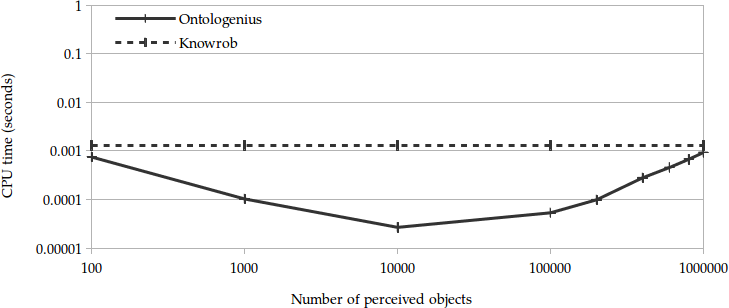
\includegraphics[width=\textwidth]{figures/chapter2/knowrob/Insertion.png}
\caption{\label{fig:chap2_knowrob_insertion} Comparison of the required CPU time for creating large numbers of object perceptions in the knowledge base. Each inserted object correspond to a visual perception entity linked to a cup, a pose matrix, and a time stamp. Ontologenius is used without the ROS communication layer to provide comparable usage and thus results.}
\end{figure}

The first test consists of creating and inserting N visual perception entities in the \acrshort{kb} and measuring the required CPU time to insert one of them Theis means that we measure the average CPU time over N insertions. For each visual perception entity, we thus have to create two entities (the visual perception entity and the perceived object), two inheritance links, two raw data, and three relations (two based on data property and one based on object property). The results are shown in figure~\ref{fig:chap2_knowrob_insertion}. KnowRobs has a constant time around 1.3ms. With Ontologenius we do not have constant time. The first decreasing part can be explained by the asynchronous Ontologenius mechanism. It looks for updates at 20hz. Consequently, we can have a delay between the moment we publish updates and the moment they are processed. The effect of the mechanism disappears with the amount of data to process since once the update mechanism started, it does not stop while data have to be processed. The general trend is thus an increase in the required CPU time. This increase can come from the fact that Ontologenius performs reasoning, like the creation of the inverse relations, at update where KnowRob resolve it at query. In addition, Ontologenius also performs consistency checking at update. However, until 1,000,000 insertions and thus 2,000,000 of entities, 2,000,000 raw data, and 5,000,000 triples (2 for inheritances and 3 for relation per perception entity), the required CPU time is under 1ms.

On the basis of the same insertions as previously, the second test consists of measuring the required memory. The results are shown in figure~\ref{fig:chap2_knowrob_memory}. For a high number of individual, Ontologenius required a bit less memory. It can be explained by the fact that it has a simplified matrix representation. In addition, no information had been provided about the initial content of the~\acrshort{kb}. Both systems, therefore, require memory in the same order of magnitude.

\begin{figure}[ht!]
\centering
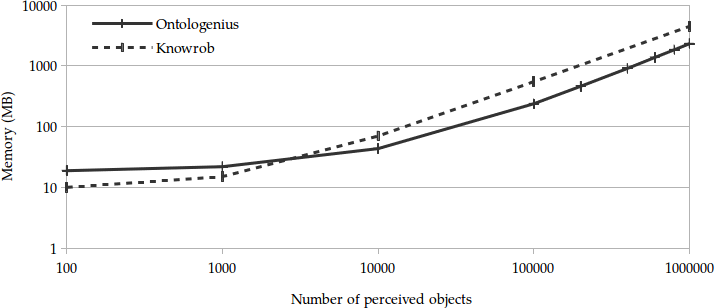
\includegraphics[width=\textwidth]{figures/chapter2/knowrob/Memory.png}
\caption{\label{fig:chap2_knowrob_memory} Comparison of the required memory for creating large numbers of object perceptions in the knowledge base. Each inserted object correspond to a visual perception entity linked to a cup, a pose matrix, and a timestamp. Ontologenius is used without the ROS communication layer to provide comparable usage and thus results.}
\end{figure}

The last test with KnowRob is about the required CPU time to perform queries. They took the same \acrshort{kb} as made previously, with N visual perception entities. The goal here is to select randomly one of the perceived cups, then retrieve its pose. In Prolog, their query is:

\paragraph{?-} owl\_individual\_of(Obj, kr:’Cup’), current\_object\_pose(Obj, Pose).

Using the low-level queries of Ontologenius, we have made a function doing the equivalent. It requests for all the cups, selects one randomly, retrieves the visual perception entity it is linked to, and fetches the pose. The required CPU time is reported in figure~\ref{fig:chap2_knowrob_query}.

\begin{figure}[ht!]
\centering
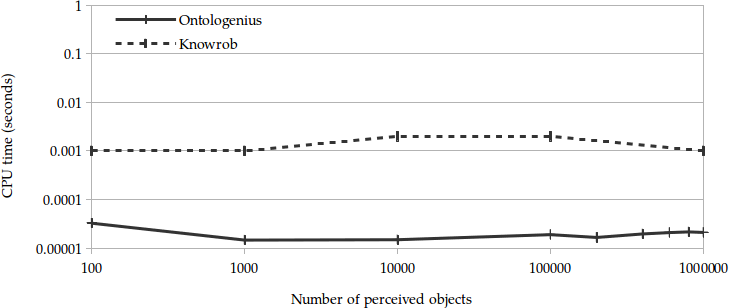
\includegraphics[width=\textwidth]{figures/chapter2/knowrob/Query.png}
\caption{\label{fig:chap2_knowrob_query} Comparison of the required CPU time for querying for the pose matrix of and randomly selected object after that N perception entities have been created. Ontologenius is used without the ROS communication layer to provide comparable usage and thus results.}
\end{figure}

Concerning KnowRob, the query time is almost constant, jumping between one and two milliseconds. It has to be noted that in Prolog, the time measurement resolution is about 1 millisecond. Nevertheless, due to the jump, we can assume that the real value is not far from the millisecond. For Ontologenius, the query time is also almost constant, with values around 0.02ms. This significant difference, with an average factor of 75, can be due to the more precise queries provided by Ontologenius and to the fact that Ontologenius does not have to solve inference at query time. For the more precise queries, submitting a query to Prolog, it has to perform a kind of search among the \acrshort{kb} to make the submitted predicates true. At the difference, Ontologenius requires the programmer to refine and decompose the high-level query, allowing the execution to be more efficient. For the inference, most of the relations are inferred at the update, like the ones coming from inverse properties. At query, Ontologenius only has to go through the existing relations and only reason about the classes and properties inclusion axioms. For example, if we had a query for all the objects, no direct link would have been created between the cups instances and the object class, this part would thus have been solved at query thanks to exploration.

In light of the presented results, even if both software have not the exact same goal, way of use, and maturity, we can at least conclude that Ontologenius is not out of scope with acceptable performance and scalability. Since Ontologenius provide fewer functionalities or at least different ones, the results are encouraging. Having poor results with fewer functionalities would have been more problematic.

\subsection{Comparing with ORO}

\subsection{Additional tests}